\chapter{Boolesches Retrieval}
Dieses Kapitel stellt das klassische Information-Retrieval-Verfahren \glqq Boolesches Retrieval\grqq{} (engl. \glqq Boolean Retrieval\grqq) vor. \\

\section{Eigenschaften des Verfahrens}
Boolesches Retrieval �berpr�ft Dokumente darauf, ob eine bestimmte Bedingung zutrifft.\\
Somit gibt es nur die Unterteilung in passende Dokumente und solche, welche die Bedingung nicht erf�llen. Eine weitere Bewertung der Ergebnisse findet nicht statt (\cite{Ferber:03}, S.33). Das fehlende Ranking der Ergebnisse ist ein h�ufiger Kritikpunkt des Verfahrens.\\
 
 
\section{Funktionsprinzip}
Boolesches Retrieval basiert auf Mengenoperationen. Deshalb werden Dokumente Mengen zugeordnet, die jeweils durch bestimmte Attribute charakterisiert sind. \\
Dokument bezeichnet die Einheit, auf welcher das Retrieval stattfindet. Ein Dokument kann deshalb eine kleine Textmemo, aber auch ein ganzes Buchkapitel sein (\cite{Manning:08}, S.4).\\
\subsection{Attribut}
Ein solches Attribut ist eine Abbildung, welche jedem Dokument einen Wert f�r dieses Attribut zuordnet. Die Abbildung erzeugt somit Attribut-Wert-Paare, was in Formel \ref{attr} gezeigt wird. 

\begin{equation}
\label{attr}
t: D \rightarrow T, t(d) = t_i
\end{equation}


Hierbei bezeichnet $t$ die Abbildung (d.h. das Attribut), $D$ die Menge aller Dokumente und $T$ den Wertebereich des Attributs $t$. \\
 Der Attributwert $t_i$ mit $t_i \in T$ und $i \in N$ wird durch die Abbildung $t$ dem Dokument $d \in D$ zugeordnet. \\

\subsection{Anfragen}

\subsubsection{Elementare boolesche Anfrage}
Ein Attribut-Wert-Paar wird auch als elementare boolesche Anfrage bezeichnet. Bei der elementaren booleschen Anfrage  $(t,t_1)$ werden zum Beispiel alle Dokumente gesucht, deren Attribut $t$ den Wert $t_1$ annimmt. \\
Mathematisch kann die Ergebnismenge $D_t,_{t_i}$ f�r eine Anfrage $(t,t_i)$ wie in Formel \ref{ergMen} beschrieben werden. 

\begin{equation}
\label{ergMen}
D_t,_{t_i} =  \{d \in D | t(d) = t_i\} \\
\end{equation}

\subsubsection{Verkn�pfung}

Mehrere Attribut-Wert-Paare lassen sich mit booleschen Operatoren $AND$, $OR$ und $NOT$ verkn�pfen. \\
$(t,t_1)$ $AND$ $(s,s_1)$ bedeutet, dass alle Dokumente gesucht sind, bei denen sowohl $t(d) = t_1$ als auch $s(d) = s_1$ gilt, d.h. hier muss der Durchschnitt dieser beiden Ergebnismengen gebildet werden, wie in Formel \ref{intersection} gezeigt.

\begin{equation}
\label{intersection}
D_t,_{t_1} \cap D_s,_{s_1}
\end{equation}


Wird hingegen der Operator $OR$ verwendet, werden die Ergebnismengen vereinigt, wie in Formel \ref{union} gezeigt. \\


\begin{equation}
\label{union}
D_t,_{t_1} \cup D_s,_{s_1}
\end{equation}


Au�erdem kann der un�re Operator $NOT$ verwendet werden, der das Komplement der Ergebnismenge erzeugt. Demnach wird f�r die Anfrage $NOT$ $(t,t_1)$ erst die Menge aller Dokumente bestimmt, bei denen $t(d) = t_1$ zutrifft, und diese anschlie�end von der Gesamtmenge aller Dokumente abgezogen. Dies wird in Formel \ref{minus} dargestellt.


\begin{equation}
\label{minus}
D \setminus D_t,_{t_1}
\end{equation}



Da bei jeder Operation neue Ergebnismengen entstehen, lassen sich hierauf erneut die oben beschriebenen Operatoren anwenden. Auf diese Weise k�nnen Anfragen beliebig tief geschachtelt werden (\cite{Ferber:03}, S.34).


\section{Indizierung}
\label{index}
Um boolesche Anfragen zu verarbeiten zu k�nnen, m�ssen die Terme der Dokumente zun�chst indiziert werden.\\
Mit \glqq Term\grqq{} wird die Einheit, welche indiziert wird, bezeichnet. Dies kann ein Wort, aber auch eine andere Einheit wie die entsprechende Stammform sein. \\
Auch die Dokumente selbst m�ssen mit einem Index versehen werden. \\
Dieses Vorgehen ist unabdingbar, da ohne Indizierung nicht effizient auf die Dokument sowie deren Terme zugriffen werden kann. Eine fehlende Indizierung w�rde bedeuten, dass f�r jede Anfrage alle Dokumente der Sammlung vollst�ndig durchlaufen werden m�ssen, was unzumutbar langsam w�re (\cite{Manning:08}, S.3).


\section{Inzidenz-Matrix}
Eine m�gliche Implementierung des Boolean Retrieval stellt die Umsetzung mittels einer Term-Dokument-Inzidenz-Matrix dar. Dies bedeutet, dass die Zeilen der Matrix die Terme enthalten und die Spalten die Dokumente, was auch umgekehrt realisierbar ist. Tritt Term $t$ in Dokument $d$ auf, so lautet der Eintrag f�r $(t,d)$ der Matrix 1. Alle Eintr�ge f�r nicht vorkommende Terme sind hingegen mit einer 0 versehen (\cite{Manning:08}, S.4). \\
Diese Herangehensweise ist belegt jedoch unn�tig viel Speicherplatz, da sehr viele Eintr�ge der Matrix eine 0 enthalten. Gerade bei sehr gro�en Sammlungen bzw. Dokumenten ist dies nicht realisierbar.

%beispiel

\subsection{Verarbeitung einer Anfrage}

\section{Invertierte Liste}
In der Regel werden zur Implementierung des Booleschen Retrieval invertierte Listen verwendet (\cite{Ferber:03}, S.36). \\
Der Name basiert auf den darin gespeicherten \glqq invertierten Indizes\grqq{}. Diese werden deshalb als invertiert bezeichnet, weil sie vom Term zur�ck auf die Postion, in welcher der Term aufgetreten ist, schlie�en lassen.\\
In einer geeigneten Speicherstruktur, zum Beispiel einem Dictionary, werden zu jedem Term alle Dokumente gespeichert, in denen der Term auftritt.\\
 Diese Dokumentlisten werden als invertierte Listen (engl. \textit{inverted lists}) bezeichnet (siehe Abbildung Abbildung \ref{abb1}). Manche Implementierungen beinhalten neben dem Dokumentindex zus�tzliche Informationen wie die genaue Wortpostion im Dokument. \\
Dieses Vorgehen setzt voraus, dass zuvor eine Indizierung (siehe \ref{index}) stattgefunden hat (\cite{Manning:08}, S.5-6). \\
Das Verfahren erm�glicht sehr schnelle Zugriffe, ist allerdings speicherintensiv (\cite{Ferber:03}, S.36). Im Vergleich zur Inzidenz-Matrix wird jedoch deutlich weniger Speicher ben�tigt, da die vielen leeren Eintr�ge entfallen.
\begin{figure} [hbtp]
	\centering
	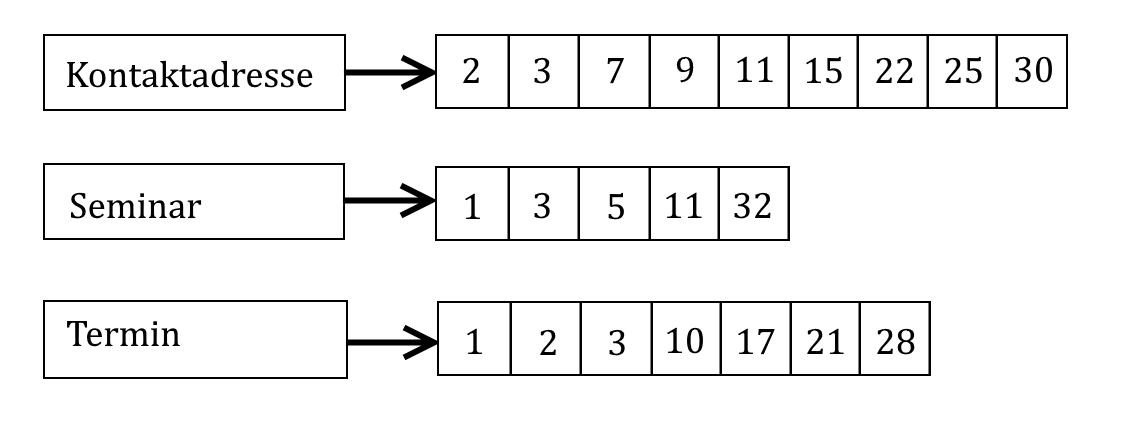
\includegraphics[width=1\textwidth]{images/inverted_list.png}
	\caption{Invertierte Listen zu Beispieltermen. Die Zahlen sind die Dokumentindizes, in denen der jeweilige Term vorkommt (Eigene Abbildung).}
	\label{abb1}
\end{figure}


%beispiel
\newpage
\subsection{Verarbeitung einer Anfrage}



